% Options for packages loaded elsewhere
\PassOptionsToPackage{unicode}{hyperref}
\PassOptionsToPackage{hyphens}{url}
%
\documentclass[
]{article}
\usepackage{amsmath,amssymb}
\usepackage{lmodern}
\usepackage{iftex}
\ifPDFTeX
  \usepackage[T1]{fontenc}
  \usepackage[utf8]{inputenc}
  \usepackage{textcomp} % provide euro and other symbols
\else % if luatex or xetex
  \usepackage{unicode-math}
  \defaultfontfeatures{Scale=MatchLowercase}
  \defaultfontfeatures[\rmfamily]{Ligatures=TeX,Scale=1}
\fi
% Use upquote if available, for straight quotes in verbatim environments
\IfFileExists{upquote.sty}{\usepackage{upquote}}{}
\IfFileExists{microtype.sty}{% use microtype if available
  \usepackage[]{microtype}
  \UseMicrotypeSet[protrusion]{basicmath} % disable protrusion for tt fonts
}{}
\makeatletter
\@ifundefined{KOMAClassName}{% if non-KOMA class
  \IfFileExists{parskip.sty}{%
    \usepackage{parskip}
  }{% else
    \setlength{\parindent}{0pt}
    \setlength{\parskip}{6pt plus 2pt minus 1pt}}
}{% if KOMA class
  \KOMAoptions{parskip=half}}
\makeatother
\usepackage{xcolor}
\IfFileExists{xurl.sty}{\usepackage{xurl}}{} % add URL line breaks if available
\IfFileExists{bookmark.sty}{\usepackage{bookmark}}{\usepackage{hyperref}}
\hypersetup{
  hidelinks,
  pdfcreator={LaTeX via pandoc}}
\urlstyle{same} % disable monospaced font for URLs
\usepackage{graphicx}
\makeatletter
\def\maxwidth{\ifdim\Gin@nat@width>\linewidth\linewidth\else\Gin@nat@width\fi}
\def\maxheight{\ifdim\Gin@nat@height>\textheight\textheight\else\Gin@nat@height\fi}
\makeatother
% Scale images if necessary, so that they will not overflow the page
% margins by default, and it is still possible to overwrite the defaults
% using explicit options in \includegraphics[width, height, ...]{}
\setkeys{Gin}{width=\maxwidth,height=\maxheight,keepaspectratio}
% Set default figure placement to htbp
\makeatletter
\def\fps@figure{htbp}
\makeatother
\setlength{\emergencystretch}{3em} % prevent overfull lines
\providecommand{\tightlist}{%
  \setlength{\itemsep}{0pt}\setlength{\parskip}{0pt}}
\setcounter{secnumdepth}{5}
\ifLuaTeX
  \usepackage{selnolig}  % disable illegal ligatures
\fi

\author{}
\date{}

\begin{document}

\title{MLT Week-8}
\author{Sherry Thomas \\ 21f3001449}

\maketitle
\tableofcontents

\begin{abstract}
This week's discussion revolves around the Naive Bayes algorithm for classification, with a comprehensive analysis of its benefits and limitations. Moreover, the session also covers the Gaussian Naive Bayes algorithm, delving into its specifics and applications.
\end{abstract}

\hypertarget{generative-model-based-algorithm}{%
\section{Generative Model Based
Algorithm}\label{generative-model-based-algorithm}}

A Generative Model Based Algorithm tries to model the probability
distribution of the input data and then generates new samples from this
distribution. It involves learning the joint probability distribution of
the features and labels of the training data, and then using this model
to make predictions for new, unseen data.

Let \(D=\{(x_1, y_1), \ldots, (x_n,y_n)\}\) be the dataset, where
\(x_i \in \{0, 1\}^d\) and \(y_i \in \{0, 1\}\).

\newpage
General Steps in the algorithm are:

\begin{itemize}
\tightlist
\item
  Decide the labels by tossing a coin \(P(y_i=1)=p\).
\item
  Decide features using the labels in step 1 using \(P(x_i|y_i)\).
\end{itemize}

The parameters in the model are as follows:

\begin{itemize}
\tightlist
\item
  Parameter \(\hat{p}\) to decide the label: 1
\item
  Parameters for \(P(x|y=1)\): \(2^d-1\)
\item
  Parameters for \(P(x|y=0)\): \(2^d-1\)
\end{itemize}

Hence, the total number of parameters \begin{align*}
    &=1 + (2^d-1) + (2^d-1)\\
    &=1 + 2(2^d-1)\\
    &=2^{d+1}-1
\end{align*}

\textbf{Issues}:

\begin{itemize}
\tightlist
\item
  Too many parameters.
\item
  Not a reasonable model.
\end{itemize}

\hypertarget{alternate-generative-model}{%
\subsection{Alternate Generative
Model}\label{alternate-generative-model}}

An alternate model begins with the class conditional independence
assumption. The \textbf{class conditional independence assumption} is a
common assumption made in machine learning algorithms that assumes the
features of an object are conditionally independent given its class
label.

Let \(D=\{(x_1, y_1), \ldots, (x_n,y_n)\}\) be the dataset, where
\(x_i \in \{0, 1\}^d\) and \(y_i \in \{0, 1\}\).

General Steps in the algorithm are:

\begin{itemize}
\tightlist
\item
  Decide the labels by tossing a coin \(P(y_i=1)=p\).
\item
  Decide features for \(x\) given \(y\) using: \[
  P(x = [f_1, f_2, \ldots, f_d]|y) = \prod_{i=1}^d(p^y_i)^{f_i}(1-p^y_i)^{1-f_i}
  \]
\end{itemize}

The parameters in the model are as follows:

\begin{itemize}
\tightlist
\item
  Parameter \(\hat{p}\) to decide the label: 1
\item
  Parameters for \(P(x|y=1)\): \(d\)
\item
  Parameters for \(P(x|y=0)\): \(d\)
\end{itemize}

Hence, the total number of parameters \begin{align*}
    &=1 + d + d\\
    &=2d+1
\end{align*}

The parameters are estimated using Maximum Likelihood Estimation.

\hypertarget{naive-bayes-algorithm}{%
\section{Naive Bayes Algorithm}\label{naive-bayes-algorithm}}

The model is given by, \[
P(x = [f_1, f_2, \ldots, f_d]|y) = \prod_{i=1}^d(p^y_i)^{f_i}(1-p^y_i)^{1-f_i}
\] The parameters to be estimated are
\(p,\{p^0_1,p^0_2,\ldots,p^0_d\},\{p^1_1,p^1_2,\ldots,p^1_d\}\). Using
Maximum Likelihood Estimation, we get the following results:
\begin{align*}
\hat{p}&=\frac{1}{n}\sum_{i=1}^ny_i\\
\hat{p}^y_j &= \frac{\displaystyle \sum_{i=1}^n\mathbb{1}(f^i_j=1,y_i=y)}{\displaystyle \sum_{i=1}^n\mathbb{1}(y_i=y)} \hspace{1em} \genfrac{}{}{0pt}{}{\forall j \in\{1,2,\ldots,d\}}{\forall y \in \{0,1\}} 
\end{align*}

\hypertarget{prediction-using-the-parameters}{%
\subsection{Prediction using the
parameters}\label{prediction-using-the-parameters}}

Given \(x^{test}\in\{0,1\}^d\), prediction for \(\hat{y}^{test}\) is
done using the following: \[
P(\hat{y}^{test}=1|x^{test}) \ge P(\hat{y}^{test}=0|x^{test})
\] If the above is true, \(\hat{y}^{test}=1\), otherwise \(0\).

Using Bayes rule, we can get the values for
\(P(\hat{y}^{test}=1|x^{test})\) and \(P(\hat{y}^{test}=0|x^{test})\):
\begin{align*}
P(\hat{y}^{test}=1|x^{test})&=\frac{P(x^{test}|\hat{y}^{test}=1)*P(\hat{y}^{test}=1)}{P(x^{test})}\\
P(\hat{y}^{test}=0|x^{test})&=\frac{P(x^{test}|\hat{y}^{test}=0)*P(\hat{y}^{test}=0)}{P(x^{test})}
\end{align*} As we predict by comparing the two values, we can do this
without actually solving for \(P(x^{test})\).

Solving for \(P(x^{test}|\hat{y}^{test}=1)*P(\hat{y}^{test}=1)\), we
get, \begin{align*}
&=P(x^{test} = [f_1, f_2, \ldots, f_d]|y^{test}=1)*P(\hat{y}^{test}=1)\\
&=\left(\prod_{i=1}^d(\hat{p}^1_i)^{f_i}(1-\hat{p}^1_i)^{1-f_i}\right)*\hat{p}
\end{align*} Similarly we solve for
\(P(x^{test}|\hat{y}^{test}=0)*P(\hat{y}^{test}=0)\).

\newpage
Therefore, if \[
\left(\prod_{i=1}^d(\hat{p}^1_i)^{f_i}(1-\hat{p}^1_i)^{1-f_i}\right)*\hat{p} \ge \left(\prod_{i=1}^d(\hat{p}^0_i)^{f_i}(1-\hat{p}^0_i)^{1-f_i}\right)*(1-\hat{p})
\] we predict \(y^{test}=1\), othewise \(y^{test}=0\).

The model implements two main things:

\begin{itemize}
\tightlist
\item
  Class Conditional Independence Assumption
\item
  Bayes Rule
\end{itemize}

Therefore, we call this algorithm Naive Bayes.

In short, \textbf{Naive Bayes} is a classification algorithm based on
Bayes' theorem, which assumes that the features are independent of each
other given the class label. It calculates the probability of a sample
belonging to a class by estimating the conditional probability of each
feature given the class and then multiplying them together using Bayes'
theorem. Despite its simple assumption, Naive Bayes is known to perform
well in various applications, particularly when there are many features
but relatively few training examples.

\hypertarget{pitfalls-of-naive-bayes}{%
\subsection{Pitfalls of Naive Bayes}\label{pitfalls-of-naive-bayes}}

The most prominent issue with Naive Bayes is that if a feature is not
seen in the training set but seen in the testing set, the prediction
probability for both the classes would be zero. \begin{align*}
P(\hat{y}^{test}=1|x^{test} = [f_1, f_2, \ldots, f_d])&\propto\left(\prod_{i=1}^d(\hat{p}^1_i)^{f_i}(1-\hat{p}^1_i)^{1-f_i}\right)*\hat{p}\\
P(\hat{y}^{test}=0|x^{test} = [f_1, f_2, \ldots, f_d])&\propto\left(\prod_{i=1}^d(\hat{p}^0_i)^{f_i}(1-\hat{p}^0_i)^{1-f_i}\right)*(1-\hat{p})
\end{align*} Even if one feature \(f_i\) was zero in training set, we
get \(\hat{p}^1_i=\hat{p}^0_i=0\), which ultimately results in
\(P(\hat{y}^{test}=0|x^{test})=P(\hat{y}^{test}=1|x^{test})=0\).

A popular fix for this is to introduce two ``pseudo'' datapoints with
labels \(1\) and \(0\) each into the dataset whose features are all
ones. This technique is also known as Laplace smoothing.

Briefly speaking, \textbf{Laplace smoothing} is a technique used to
address the zero-frequency problem in probabilistic models, particularly
in text classification. It involves adding a small constant value to the
count of each feature and the number of unique classes to avoid zero
probability estimates, which can cause problems during model training
and prediction. By adding this smoothing term, the model becomes more
robust and can handle unseen data more effectively.

\hypertarget{decision-function-of-naive-bayes}{%
\section{Decision Function of Naive
Bayes}\label{decision-function-of-naive-bayes}}

\begin{multline*}
\text{Given } x^{test}\in\{0,1\}^d \text{, prediction for }\hat{y}^{test} \text{ is } 1\text{ if:}\\
\frac{P(\hat{y}^{test}=1|x^{test})}{P(\hat{y}^{test}=0|x^{test})}\ge 1\\
\log \left (\frac{P(\hat{y}^{test}=1|x^{test})}{P(\hat{y}^{test}=0|x^{test})}\right )\ge 0\\
\log \left (\frac{\displaystyle\frac{P(x^{test}|\hat{y}^{test}=1)*P(\hat{y}^{test}=1)}{P(x^{test})}}{\displaystyle\frac{P(x^{test}|\hat{y}^{test}=0)*P(\hat{y}^{test}=0)}{P(x^{test})}}\right )\ge 0 \\
\log \left (\prod_{i=1}^d\frac{(\hat{p}^1_i)^{f_i}(1-\hat{p}^1_i)^{1-f_i}\hat{p}}{(\hat{p}^0_i)^{f_i}(1-\hat{p}^0_i)^{1-f_i}(1-\hat{p})}\right )\ge 0 \\
\log \left (\prod_{i=1}^d\left(\frac{\hat{p}^1_i}{\hat{p}^0_i}\right)^{f_i}\left(\frac{1-\hat{p}^1_i}{1-\hat{p}^0_i}\right)^{1-f_i}\frac{\hat{p}}{1-\hat{p}}\right )\ge 0 \\
\sum_{i=1}^d \left (f_i\log\left(\frac{\hat{p}^1_i}{\hat{p}^0_i}\right)+(1-f_i)\log\left(\frac{1-\hat{p}^1_i}{1-\hat{p}^0_i}\right)+\log\left(\frac{\hat{p}}{1-\hat{p}}\right)\right )\ge 0 \\
\sum_{i=1}^d \left (f_i\log\left(\frac{\hat{p}^1_i(1-\hat{p}^0_i)}{\hat{p}^0_i(1-\hat{p}^1_i)}\right)\right )+\sum_{i=1}^d\log\left(\frac{1-\hat{p}^1_i}{1-\hat{p}^0_i}\right)+\log\left(\frac{\hat{p}}{1-\hat{p}}\right)\ge 0 \\
\end{multline*} Hence, we can say that the decision function is of the
form \(w^Tx+b\ge0\) where \(w\in\mathbb{R}^d\),
\(w_i=\displaystyle\log\left(\frac{\hat{p}^1_i(1-\hat{p}^0_i)}{\hat{p}^0_i(1-\hat{p}^1_i)}\right)\)
and
\(b=\displaystyle\sum_{i=1}^d\log\left(\frac{1-\hat{p}^1_i}{1-\hat{p}^0_i}\right)+\log\left(\frac{\hat{p}}{1-\hat{p}}\right)\).

Therefore, the decision function of Naive Bayes is \textbf{Linear}.

The decision boundary is given by \(\{x=P(y=1|x)=P(y=0|x)\}\).

\hypertarget{gaussian-naive-bayes}{%
\section{Gaussian Naive Bayes}\label{gaussian-naive-bayes}}

Let \(D=\{(x_1, y_1), \ldots, (x_n,y_n)\}\) be the dataset, where
\(x_i \in \mathbb{R}^d\) and \(y_i \in \{0, 1\}\).

Let \(P(x|y=1)\sim\mathcal{N}(\mu_1,\Sigma)\) and
\(P(x|y=0)\sim\mathcal{N}(\mu_0,\Sigma)\). We assume that the
covariances are equal.

The parameters to be estimated are \(\hat{p}\), \(\mu_0\), \(\mu_1\),
and \(\Sigma\).

Using Maximum Likelihood Estimation, we get the following results:
\begin{align*} 
\hat{p}&=\frac{1}{n}\sum_{i=1}^ny_i \\
\hat{\mu_1} &= \frac{\displaystyle \sum_{i=1}^n\mathbb{1}(y_i=1)*x_i}{\displaystyle \sum_{i=1}^n\mathbb{1}(y_i=1)} \\
\hat{\mu_0} &= \frac{\displaystyle \sum_{i=1}^n\mathbb{1}(y_i=0)*x_i}{\displaystyle \sum_{i=1}^n\mathbb{1}(y_i=0)} \\
\hat{\Sigma} &= \frac{1}{n} \displaystyle \sum_{i=1}^n(x_i-\hat{\mu}_{y_i})(x_i-\hat{\mu}_{y_i})^T
\end{align*} Where \(\hat{p}\) is the proportion of data points labeled
\(1\), \(\hat{\mu_1}\) is the sample mean of data points labeled \(1\),
\(\hat{\mu_0}\) is the sample mean of data points labeled \(0\), and
\(\hat{\Sigma}\) is covariance matrix of the centered dataset.

\hypertarget{prediction-using-bayes-rule}{%
\subsection{Prediction using Bayes
Rule}\label{prediction-using-bayes-rule}}

Prediction is based on the following equation: \[
P(y_{test}=1|x_{test})\propto P(x_{test}|y_{test})*P(y_{test})
\] where
\(P(x_{test}|y_{test})\equiv f(x_{test};\hat{\mu}_{y_{test}}, \hat{\Sigma})\)
and \(P(y_{test})\equiv \hat{p}\).

Predict \(y_{test}=1\) if: \begin{align*}
f(x_{test};\hat{\mu}_1, \hat{\Sigma})*\hat{p}&\ge f(x_{test};\hat{\mu}_0, \hat{\Sigma})*(1-\hat{p}) \\
e^{-(x_{test}-\hat{\mu}_1)^T\hat{\Sigma}(x_{test}-\hat{\mu}_1)}*\hat{p}&\ge e^{-(x_{test}-\hat{\mu}_0)^T\hat{\Sigma}(x_{test}-\hat{\mu}_0)}*(1-\hat{p}) \\
-(x_{test}-\hat{\mu}_1)^T\hat{\Sigma}(x_{test}-\hat{\mu}_1)+\log(\hat{p})&\ge -(x_{test}-\hat{\mu}_0)^T\hat{\Sigma}(x_{test}-\hat{\mu}_0) + \log(1-\hat{p}) \\
\end{align*} \[
\left( (\hat{\mu}_1-\hat{\mu}_0)^T\hat{\Sigma}^{-1} \right)x_{test} + \hat{\mu}_0^T\hat{\Sigma}^{-1}\hat{\mu}_0 - \hat{\mu}_1^T\hat{\Sigma}^{-1}\hat{\mu}_1 + log(\frac{1-\hat{p}}{\hat{p}}) \ge 0
\] Hence, we can say that the decision function is of the form
\(w^Tx+b\ge0\) where \(w\in\mathbb{R}^d\),
\(w_i= (\hat{\mu}_1-\hat{\mu}_0)^T\hat{\Sigma}^{-1}\) and
\(b=\hat{\mu}_0^T\hat{\Sigma}^{-1}\hat{\mu}_0 - \hat{\mu}_1^T\hat{\Sigma}^{-1}\hat{\mu}_1 + log(\frac{1-\hat{p}}{\hat{p}})\).

Therefore, the decision function of Gaussian Naive Bayes when the
covariance matrix is equal for both classes is \textbf{Linear}.

\hypertarget{decision-boundaries-for-different-covariances}{%
\subsection{Decision Boundaries for Different
Covariances}\label{decision-boundaries-for-different-covariances}}

\begin{enumerate}
\def\labelenumi{\arabic{enumi}.}
\tightlist
\item
  \textbf{When the covariance matrices are equal for both classes}: As
  seen previously, the decision boundary is linear.

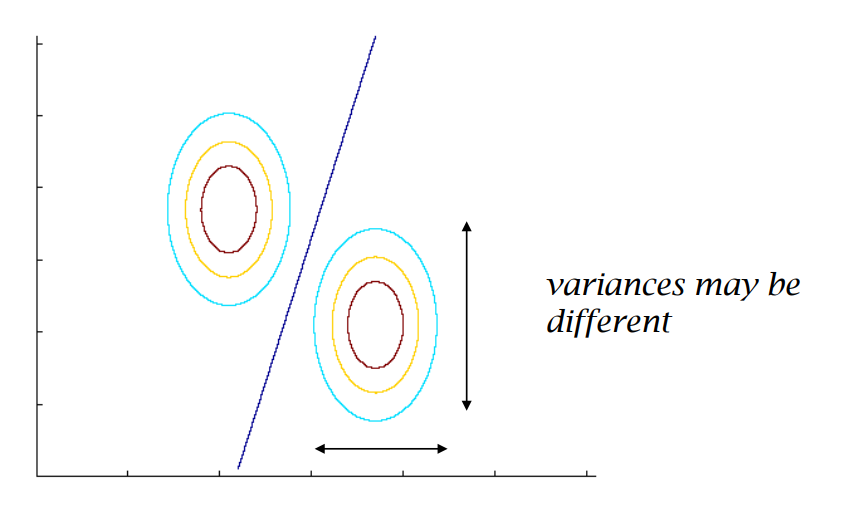
\includegraphics[width=10cm]{./images/equal_var.png} 

\item 
    \textbf{When the covariance
matrices are Identity matrices for both classes}: The decision boundary
is linear as well as the perpendicular bisector of the line drawn from
\(\hat{\mu}_1\) to \(\hat{\mu}_0\).

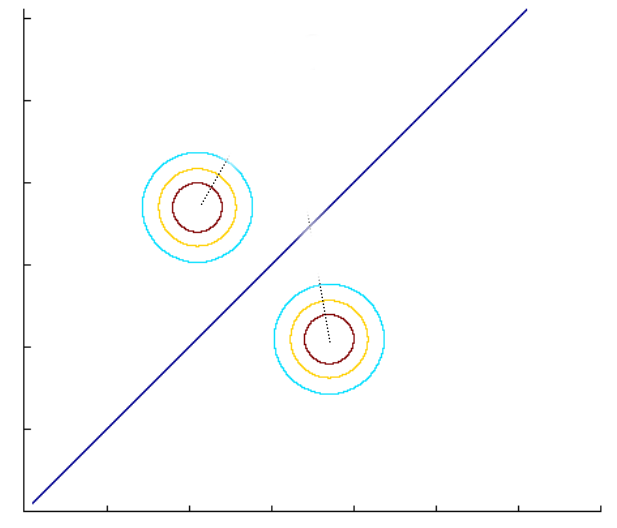
\includegraphics[width=10cm]{./images/identity_var.png}
\newpage
\item  
\textbf{When the
covariance matrices are not equal for both classes}: Let
\(\hat{\Sigma}_1\) and \(\hat{\Sigma}_0\) be the covariance matrices for
classes \(1\) and \(0\) respectively. They are given by, \begin{align*} 
\hat{\Sigma}_1 &= \frac{1}{n} \displaystyle \sum_{i=1}^n(\mathbb{1}(y_i=1)*x_i-\hat{\mu}_1)(\mathbb{1}(y_i=1)*x_i-\hat{\mu}_1)^T \\
\hat{\Sigma}_0 &= \frac{1}{n} \displaystyle \sum_{i=1}^n(\mathbb{1}(y_i=0)*x_i-\hat{\mu}_0)(\mathbb{1}(y_i=0)*x_i-\hat{\mu}_0)^T
\end{align*} Predict \(y_{test}=1\) if: \begin{align*}
f(x_{test};\hat{\mu}_1, \hat{\Sigma_1})*\hat{p}&\ge f(x_{test};\hat{\mu}_0, \hat{\Sigma_0})*(1-\hat{p}) \\
e^{-(x_{test}-\hat{\mu}_1)^T\hat{\Sigma_1}(x_{test}-\hat{\mu}_1)}*\hat{p}&\ge e^{-(x_{test}-\hat{\mu}_0)^T\hat{\Sigma_1}(x_{test}-\hat{\mu}_0)}*(1-\hat{p}) \\
-(x_{test}-\hat{\mu}_1)^T\hat{\Sigma_1}(x_{test}-\hat{\mu}_1)+\log(\hat{p})&\ge -(x_{test}-\hat{\mu}_0)^T\hat{\Sigma_0}(x_{test}-\hat{\mu}_0) + \log(1-\hat{p})
\end{align*} \[
x_{test}^T(\hat{\Sigma}_1^{-1}-\hat{\Sigma}_0^{-1})x_{test}-2(\hat{\mu}_1^T\hat{\Sigma}_1^{-1}-\hat{\mu}_0^T\hat{\Sigma}_0^{-1})x_{test}+(\hat{\mu}_0^T\hat{\Sigma}_0^{-1}\hat{\mu}_0-\hat{\mu}_1^T\hat{\Sigma}_1^{-1}\hat{\mu}_1) + log(\frac{1-\hat{p}}{\hat{p}}) \ge 0
\] Hence, we can say that the decision function is of the form
\(x^TQx-2b^Tx+c\ge0\) where
\(Q=\hat{\Sigma}_1^{-1}-\hat{\Sigma}_0^{-1}\),
\(b=\hat{\mu}_1^T\hat{\Sigma}_1^{-1}-\hat{\mu}_0^T\hat{\Sigma}_0^{-1}\),
and
\(c=(\hat{\mu}_0^T\hat{\Sigma}_0^{-1}\hat{\mu}_0-\hat{\mu}_1^T\hat{\Sigma}_1^{-1}\hat{\mu}_1) + log(\frac{1-\hat{p}}{\hat{p}})\).

Hence, the decision boundary is a quadratic function when the covariance
matrices are not equal for both classes.

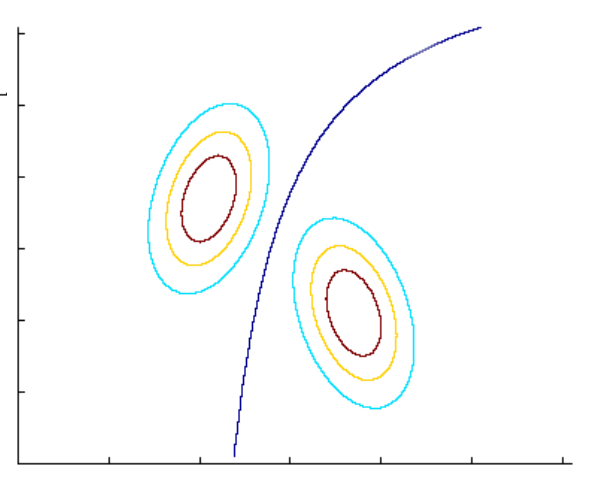
\includegraphics[width=10cm]{./images/non-equal_var.png}

\end{enumerate}

\hypertarget{credits}{%
\section{Credits}\label{credits}}

Professor Arun Rajkumar: The content as well as the notations are from
his slides and lecture.

\end{document}
